\chapter{\babEmpat}
\label{bab:4}

Bab ini membahas mengenai proses \f{fine tuning} model \f{Bidirectional Encoder Representations from Transformers} (BERT) untuk mendapatkan model yang dapat digunakan untuk masalah pemeringkatan teks.
\sect\ref{sec:spesifikasi} menjelaskan mengenai spesifikasi perangkat keras dan perangkat lunak yang digunakan dalam penelitian. Selanjutnya, \sect~\ref{sec:simulasi} menjelaskan mengenai tahapan simulasi yang dilakukan dalam penelitian. Informasi mengenai \f{dataset} latih dan uji  dijelaskan pada \sect~\ref{sec:dataset}. \sect~\ref{sec:finetuning} menjelaskan lebih detail mengenai arsitektur model BERT, fungsi loss, serta konfigurasi \f{hyperparameter} yang digunakan dalam proses \f{fine tuning} model BERT. Terakhir, \sect~\ref{sec:hasil} menjelaskan mengenai evaluasi hasil \f{fine tuning} model BERT untuk pemeringkatan teks.

\section{Spesifikasi Mesin dan Perangkat Lunak}
\label{sec:spesifikasi}

Proses \f{fine tuning} model BERT untuk pemeringkatan teks dilakukan menggunakan mesin dan perangkat lunak yang tertera pada \tab~\ref{tab:spesifikasi}.
\begin{table}[!ht]
    \centering
    \caption{Spesifikasi Perangkat Lunak}
    \label{tab:spesifikasi}
    \begin{tabular}{|l|l|} \hline
        \textbf{CPU}                         & AMD Ryzen 9 5950X 32-Core Processor                                                                                                      \\ \hline
        \textbf{GPU}                         & NVIDIA GeForce RTX 4090 24GB                                                                                                             \\ \hline
        \textbf{Memori}                      & 64GB                                                                                                                                     \\ \hline
        \textbf{Sistem Operasi}              & Ubuntu 20.04.2 LTS                                                                                                                       \\ \hline
        \textbf{Perangkat Lunak Pemrograman} & Visual Studio Code 1.84.2                                                                                                                \\ \hline
        \textbf{Bahasa Pemrograman}          & Python 3.8                                                                                                                               \\ \hline
        \textbf{Pustaka yang Digunakan}      & \begin{tabular}[c]{@{}l@{}}sentence-transformers 2.2.2\\ transformers 4.35.1\\ beir 2.0.0\\ gdown 4.7.1\\ torch 2.0.1+cu117\end{tabular} \\ \hline
    \end{tabular}
\end{table}

\section{Tahapan Simulasi}
\label{sec:simulasi}

\pic~\ref{fig:diagram-simulasi} menunjukkan tahapan simulasi yang dilakukan dalam penelitian ini.
\begin{figure}
    \centering
    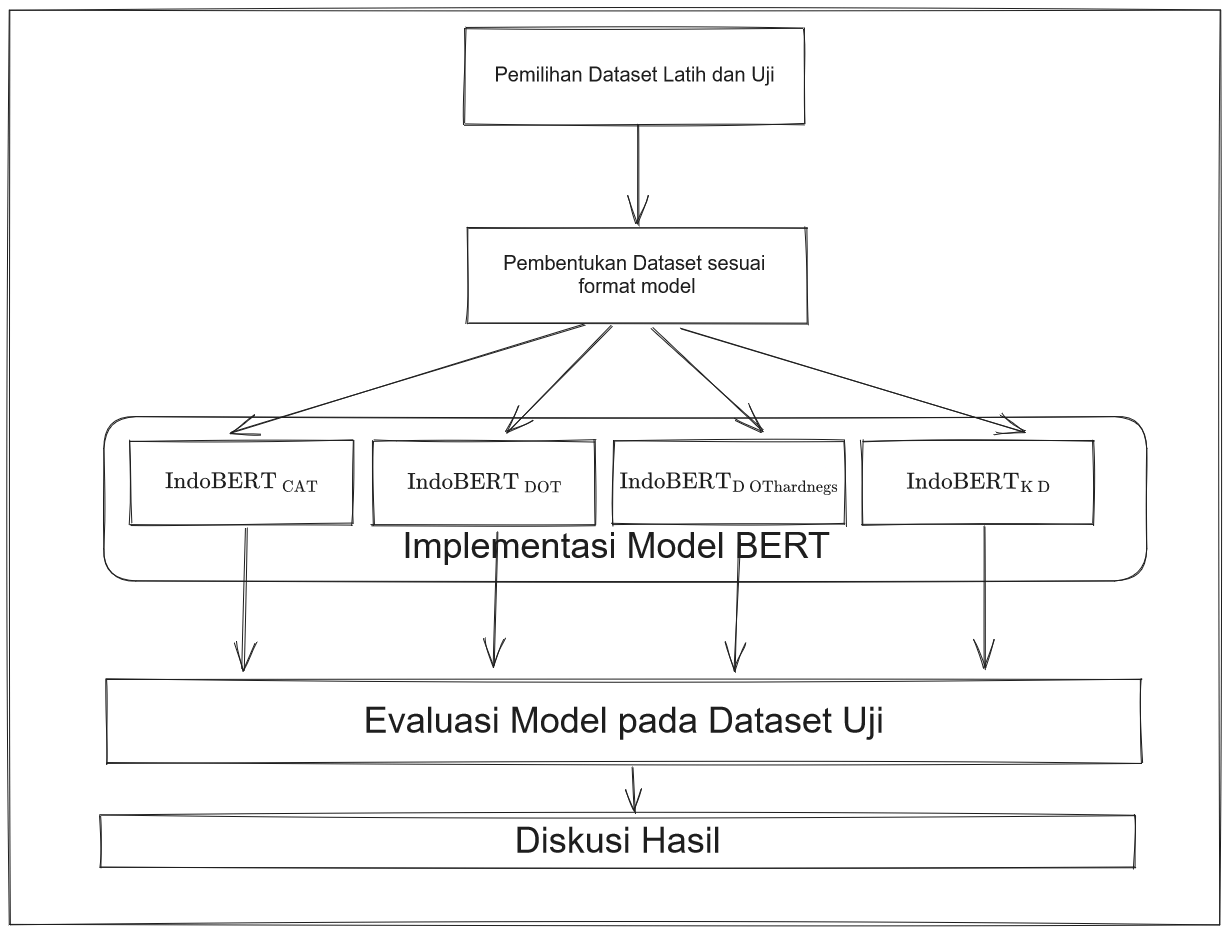
\includegraphics[width=1\textwidth]{assets/pics/alursimulasi.png}
    \caption{Diagram Simulasi}
    \label{fig:diagram-simulasi}

\end{figure}

Simulasi diawali dengan pengambilan data. Data yang digunakan adalah data pada penelitian \cite{mmarco}, sebagai \f{dataset} latih, dan data pada penelitian \cite{mrtydi}, \cite{miracl} sebagai \f{dataset} ujinya. \f{Dataset} latih tidak dapat digunakan langsung untuk melatih model-model tersebut. Untuk setiap modelnya, diperlukan transformasi untuk mengubah bentuk dari \f{dataset} latih sehingga sesuai dengan formatnya. Transformasi \f{dataset} latih dan \f{hyperparameter} dari model akan dibahas lebih lanjut pada bagian \sect~\ref{sec:finetuning}. Selanjutnya, proses implementasi dan pelatihan model dilakukan. Setelah itu, Evaluasi dari setiap model pada \f{dataset} uji dilakukan. Terdapat satu model BM25 sebagai \f{baseline} untuk setiap modelnya. Terakhir, terdapat diskusi mengenai hasil evaluasi tersebut.

\section{Data}
\label{sec:dataset}

Penelitian ini menggunakan satu \f{dataset} latih Mmarco train set Indonesia \citep{mmarco} dan tiga \f{dataset} uji, yaitu Mmarco Dev set Indonesia, MrTyDi Test set Indonesia \citep{mrtydi}, dan Miracl Dev set Indonesia \citep{miracl}. \f{Dataset} Miracl dan MrTyDi dipilih sebagai uji kemampuan \f{out-of-distibution} dari model yang dihasilkan. \f{Dataset} tersebut terdiri dari 3 file, yaitu \f{file} kueri, \f{file korpus} dan \f{file jugdements} yang telah dijelaskan pada \sect~\ref{sec:dataset-umum}. \tab~\ref{tab:dataset-info} menunjukkan informasi mengenai jumlah entri dari \f{file} kueri, \f{file korpus}, dan \f{file jugdements} dari setiap \f{dataset} yang digunakan dalam penelitian ini. Setiap \f{judgements} pada \f{dataset} adalah \f{jugdments} biner, yaitu bernilai 1 jika dokumen tersebut relevan dengan kueri dan 0 jika tidak relevan dengan kueri. \pic~\ref{fig:dataset-mircal-judgments} menunjukkan contoh \f{file jugdements} dari \f{dataset} Miracl Dev set Indonesia.


\begin{table}[!ht]
    \centering
    \caption{Dataset Information}
    \label{tab:dataset-info}
    \begin{tabular}{|l|c|c|c|} \hline
        \textbf{Dataset} & \textbf{Korpus} & \textbf{Kueri} & \textbf{Jugdements} \\ \hline
        Mmarco train set & 8,841,823       & 1,010,916      & 532,761             \\ \hline
        Mmarco dev set   & 8,841,823       & 1,010,916      & 7,437               \\ \hline
        Mrtydi test set  & 1,469,399       & 829            & 961                 \\ \hline
        Miracl dev set   & 1,446,315       & 960            & 9,668               \\ \hline
    \end{tabular}
\end{table}

\section{Fine Tuning Model BERT}
\label{sec:finetuning}


\subsection{$\text{IndoBERT}_{\text{CAT}}$}


Pada model $\text{IndoBERT}{\text{CAT}}$, arsitektur $\text{BERT}\text{CAT}$ (lihat \sect~\ref{sec:bert-cat}) digunakan untuk melakukan pemeringkatan teks. Selama proses pelatihan model, \f{dataset} yang digunakan berasal dari Mmarco train set dengan format $(q, d, r)$ dengan $q$ adalah kueri, $d$ adalah dokumen, dan $r$ adalah relevansi dokumen $d$ terhadap kueri $q$. Pelatihan yang dilakukan adalah pelatihan untuk klasifikasi relevansi dokumen terhadap kueri. Perlu dicatat bahwa tidak ada contoh $r=0$ dalam \f{dataset} Mmarco train set (lihat \sect~\ref{sec:dataset-umum}).

Untuk membentuk data latih dengan penilaian $r=0$, pasangan $(q, d',0)$ ditambahkan dengan $d'$ sebagai dokumen acak yang tidak relevan dengan kueri $q$. \f{Dataset} yang telah dibuat terdiri dari 500 ribu pasangan $(q, d, r)$ dengan rasio 1:1 antara $r=1$ dan $r=0$. contoh dari \f{dataset} yang digunakan untuk pelatihan model $\text{IndoBERT}_{\text{CAT}}$ dapat ditemukan pada \tab~\ref{tab:converted-table}.

\begin{table}[!ht]
    \centering
    \caption{Converted Table}
    \label{tab:converted-table}
    \begin{tabular}{|p{2cm}|p{7cm}|c|} \hline
        \textbf{Kueri}                                         & \textbf{Teks}                                                                                                                                                                                                                                                                                                                                                                                                                                                                                                                                                                                             & \textbf{Relevansi} \\ \hline
        Berapa banyak kalori sehari yang hilang saat menyusui? & Tidak hanya menyusui lebih baik untuk bayi, namun penelitian juga mengatakan itu lebih baik bagi ibu. Menyusui membakar rata-rata 500 kalori sehari, dengan kisaran khas antara 200 hingga 600 kalori yang terbakar sehari. Diperkirakan produksi 1 oz. ASI membakar 20 kalori. Jumlah kalori yang terbakar tergantung pada seberapa banyak bayi makan. Menyusui kembar membakar dua kali lebih banyak daripada memberi makan hanya satu bayi. Dengan anak kembar, ibu mereka membakar 1000 kalori per hari. Membakar 500 kalori ekstra sehari akan menghasilkan satu pon penurunan berat badan mingguan. & 1                  \\ \hline
        Karakteristik iklim utama hutan hujan tropis           & Kacang kola adalah buah dari pohon kola, genus (Cola) pohon yang berasal dari hutan hujan tropis Afrika.                                                                                                                                                                                                                                                                                                                                                                                                                                                                                                  & 0                  \\ \hline
        Berapa lama pemulihan dari humerus yang patah?         & Pemulihan Stroke. Stroke mempengaruhi setiap orang secara berbeda. Banyak penderita stroke yang terus membaik dalam waktu yang lama, kadang-kadang selama beberapa tahun. Pemulihan dari stroke melibatkan membuat perubahan dalam aspek fisik, sosial dan emosional hidup Anda. Anda akan membuat perubahan untuk mencegah stroke tambahan serta untuk memfasilitasi pemulihan seumur hidup Anda.                                                                                                                                                                                                        & 0                  \\ \hline
    \end{tabular}
\end{table}

konfigurasi \f{hyperparameter} selama pelatiahan model $\text{indoBERT}_{\text{CAT}}$ dapat  dilihat pada \tab~\ref{tab:indobert-cat-hyperparameter}.

\begin{table}[!ht]
    \centering
    \caption{Hyperparameter $\text{IndoBERT}_{\text{CAT}}$}
    \label{tab:indobert-cat-hyperparameter}
    \begin{tabular}{|c|c|}
        \hline
        \textbf{Parameter}       & \textbf{Nilai}                                                                                    \\
        \hline
        Model pralatih           & \href{https://huggingface.co/indolem/indobert-base-uncased}{\code{indolem/indobert-base-uncased}} \\
        \hline
        Total data               & 500,000                                                                                           \\
        \f{Batch Size}           & 32                                                                                                \\
        \hline
        Total iterasi            & 78125 (5 epochs)                                                                                  \\
        \hline
        \f{Optimizer}            & Adam dengan $\beta_1 = 0.9$, $\beta_2 = 0.999$, $\epsilon = 1e-8$                                 \\
        \hline
        \f{Learning rate}        & 2e-5                                                                                              \\
        \hline
        \f{Learning rate warmup} & Linear dengan 10\% dari total iterasi                                                             \\
        \hline
        Fungsi loss              & \f{Binary cross entropy}                                                                          \\
        \hline
    \end{tabular}
\end{table}



\subsection{$\text{IndoBERT}_{\text{DOT}}$}

Pada model $\text{IndoBERT}_{\text{DOT}}$, arsitektur $\text{BERT}_\text{DOT}$ (lihat \sect~\ref{sec:bert-dot}) digunakan untuk melakukan pemeringkatan teks. fungsi loss yang digunakan untuk pelatihan model $\text{IndoBERT}_{\text{DOT}}$ adalah \f{N-pair loss}. Untuk kueri $q$, dokumen relevan $d^+$, dan kumpulan dokumen tidak relevan $\{d_i^-\}_{i=1}^{n-1}$ terhadap kueri $q$, \f{N-pair loss} didefinisikan sebagai berikut:

\begin{align}
    L(q, d^+,\{d_i^-\}_{i=1}^{N-1}) = -\log \frac{\exp(\mathbf{h}^{\top}_q \mathbf{h}^+_d)}{\exp(\mathbf{h}^{\top}_q \mathbf{h}^+_d) + \sum_{i=1}^{n-1} \exp(\mathbf{h}^{\top}_q \mathbf{h}^-_i)},
\end{align}
dengan keterangan sebagai berikut:
\begin{flalign*}
    \mathbf{h}_q   & = \text{IndoBERT}_{\text{DOT}}((\text{[CLS]}, q, \text{[SEP]}))_{\text{[CLS]}}   \\
    \mathbf{h}^+_d & = \text{IndoBERT}_{\text{DOT}}(\text{[CLS]}, d^+, \text{[SEP]})_{\text{[CLS]}}   \\
    \mathbf{h}^-_i & = \text{IndoBERT}_{\text{DOT}}(\text{[CLS]}, d^-_i, \text{[SEP]})_{\text{[CLS]}}
\end{flalign*}

\f{dataset} Mmarco train set langsung dapat digunakan karena \f{dataset} tersebut sudah dalam bentuk $(q, d^+)$. Kumpulan teks tak relevan $\{d_i^-\}_{i=1}^{n-1}$ dibentuk dengan menggunakan teks $d$ pada \f{data point} yang lain pada batch yang sama. dengan begitu, nilai $N$ pada \f{N-pair loss} adalah ukuran batch yang digunakan selama pelatihan model. Metode pemilihan dokumen negatif ini disebut dengan \f{in-batch negative sampling} \citep{dprmeta}. Pada penelitian ini, digunakan seluruh \f{datapoint} pada \f{file jugdements} Mmarco train set -- 532,761 \f{data point} -- untuk membentuk \f{dataset} latih model $\text{IndoBERT}_{\text{DOT}}$.

Konfigurasi \f{hyperparameter} selama pelatiahan model $\text{indoBERT}_{\text{DOT}}$ dapat  dilihat pada \tab~\ref{tab:indobert-dot-hyperparameter}.
\begin{table}[!ht]
    \centering
    \caption{\f{Hyperparameter} $\text{IndoBERT}_{\text{DOT}}$}
    \label{tab:indobert-dot-hyperparameter}
    \begin{tabular}{|c|c|}
        \hline
        \textbf{Parameter}       & \textbf{Nilai}                                                                                    \\
        \hline
        Model pralatih           & \href{https://huggingface.co/indolem/indobert-base-uncased}{\code{indolem/indobert-base-uncased}} \\
        \hline
        \f{Batch Size}           & 32                                                                                                \\
        \hline
        Total Iterasi            & 83243 (5 epochs)                                                                                  \\
        \hline
        \f{Optimizer}            & Adam dengan $\beta_1 = 0.9$, $\beta_2 = 0.999$, $\epsilon = 1e-8$                                 \\
        \hline
        \f{Learning rate}        & 2e-5                                                                                              \\
        \hline
        \f{Learning rate warmup} & Linear dengan 10\% dari total iterasi                                                             \\
        \hline
        Fungsi \f{loss}          & \f{N-pair loss}                                                                                   \\
        \hline
    \end{tabular}
\end{table}

\subsection{$\text{IndoBERT}_{\text{DOThardnegs}}$}

Pada $\text{IndoBERT}_\text{DOThardnegs}$, arsitektur $\text{BERT}_\text{DOT}$ digunakan untuk melakukan pemeringkatan teks. fungsi loss yang digunakan untuk pelatihan model $\text{IndoBERT}_{\text{DOThardnegs}}$ adalah \f{N-pair loss} seperti $\text{IndoBERT}_{\text{DOT}}$. Perbedaan utama antara $\text{IndoBERT}_{\text{DOT}}$ dan $\text{IndoBERT}_{\text{DOThardnegs}}$ adalah metode pemilihan dokumen negatif. Pada $\text{IndoBERT}_{\text{DOT}}$, dokumen negatif dipilih dari \f{data point} lain pada batch yang sama. Pada $\text{IndoBERT}_{\text{DOThardnegs}}$, dokumen negatif sudah terlebih dahulu dipilih dengan kriteria bahwa dokumen tersebut adalah dokumen yang tidak relevan dengan kueri $q$, tetapi pemeringkatan dengan BM25 berada di 100 teratas. Dengan kata lain, dokumen negatif adalah dokumen yang sulit dibedakan dengan dokumen positif menggunakan BM25. Dokumen \f{hard negative} ini diberikan oleh file \href{https://huggingface.co/datasets/sentence-transformers/msmarco-hard-negatives}{\code{sentence-transformers/msmarco-hard-negatives}} \citep{beir} dan \tab~\ref{tab:hardnegsbm25} menunjukkan contoh dari dokumen \f{file} tersebut. Nilai $N$ yang dipilih pada penelitian ini adalah $N=5$, dan jumlah data yang digunakan adalah 502.939 \f{data point}.

\begin{table}[!ht]
    \centering
    \caption{Potongan dari \f{file} \code{sentence-transformers/msmarco-hard-negatives}. kolom qid berisikan id dari kueri, kolom \f{positive} adalah id dokumen positif, dan kolom \f{hard negative} adalah id dokumen yang sulit dibedakan dengan dokumen positif menggunakan BM25.}
    \label{tab:hardnegsbm25}
    \begin{tabular}{|c|c|p{8cm}|}
        \hline
        qid & \f{Positive} & \f{Hard Negative}                                           \\
        \hline
        634 & 1668221      & \{ "bm25": [830424, 1985345, 1153265, 1638798, 2866545] \}  \\
        \hline
        492 & 875          & \{ "bm25": [1147445, 4859158, 7980570, 3409840, 6889336] \} \\
        \hline
    \end{tabular}
\end{table}

Konfigurasi \f{hyperparameter} selama pelatiahan model $\text{indoBERT}_{\text{DOThardnegs}}$ dapat  dilihat pada \tab~\ref{tab:indobert-dothardnegs-hyperparameter}.

\begin{table}[!ht]
    \centering
    \caption{\f{Hyperparameter} $\text{IndoBERT}_{\text{DOThardnegs}}$}
    \label{tab:indobert-dothardnegs-hyperparameter}
    \begin{tabular}{|c|c|}
        \hline
        \textbf{Parameter}       & \textbf{Nilai}                                                                                    \\
        \hline
        Model pralatih           & \href{https://huggingface.co/indolem/indobert-base-uncased}{\code{indolem/indobert-base-uncased}} \\
        \hline
        Total data               & 502,939                                                                                           \\
        \hline
        \f{Batch Size}           & 32                                                                                                \\
        \hline
        Total Iterasi            & 78585 (5 epochs)                                                                                  \\
        \hline
        \f{Optimizer}            & Adam dengan $\beta_1 = 0.9$, $\beta_2 = 0.999$, $\epsilon = 1e-8$                                 \\
        \hline
        \f{Learning rate}        & 2e-5                                                                                              \\
        \hline
        \f{Learning rate warmup} & Linear dengan 10\% dari total iterasi                                                             \\
        \hline
        Fungsi \f{loss}          & \f{N-pair loss}                                                                                   \\
        \hline
    \end{tabular}
\end{table}

\subsection{$\text{IndoBERT}_{\text{DOTMargin}}$}


\subsection{$\text{IndoBERT}_{\text{DOTKD}}$}
$\text{IndoBERT}_{\text{KD}}$ dilatih dengan menggunakan prinsip \f{knowledge distillation}, yaitu proses \f{transfer} pengetahuan dari model yang sudah dilatih dengan baik (guru) ke model yang belum dilatih (murid). Model yang digunakan sebagai guru adalah model bahasa Inggris yang sudah dilatih dengan baik untuk melakukan pemeringkatan teks. Model Murid harus dipilih adalah model pralatih BERT multibahasa -- model yang \f{pre-training}-nya dilakukan pada korpus multibahasa. Pemetaaan vektor dari model murid akan di-\f{align} dengan Pemetaan vektor dari model guru dengan fungsi \f{loss} berikut \citep{knowledgedistill}:
\begin{align}
    L(s_i, t_i) = \left(\mid \mid M(s_i) - \hat{M}(s_i) \mid \mid + \mid\mid M(s_i) - \hat{M}(s_) \mid\mid \right),
\end{align}
dengan keterangan sebagai berikut:
\begin{flalign*}
    M        &= \text{model guru (bahasa Inggris)}&& \\
    \hat{M}  &= \text{model pralatih BERT murid (multibahasa)}&& \\
    s_i      &= \text{teks sumber (bahasa Inggris)}&& \\
    t_i      &= \text{teks target (bahasa Indonesia)}&&
\end{flalign*}




\section{Hasil Fine Tuning dan Evaluasi}
\label{sec:hasil}

\subsection{Evaluasi BM25}
\label{sec:resultbm25}

\begin{table}[!ht]
    \centering
    \caption{Caption}
    \label{tab:bm25-result}
    \begin{tabular}{|c|cc|cc|cc|} \hline
        Model                             & \multicolumn{2}{|c|}{Mmarco Dev} &
        \multicolumn{2}{|c|}{MrTyDi Test} & \multicolumn{2}{|c|}{Miracl Dev}                                             \\ \hline
                                          & MRR@10                           & R@1000 & MRR@10 & R@1000 & NCDG@10 & R@1K \\ \hline
        BM25 (Elastic Search)             & .114                             & .642   & .279   & .858   & .391    & .971 \\ \hline
    \end{tabular}
\end{table}

\subsection{Evaluasi $\text{IndoBERT}_{\text{MEAN}}$}
\label{sec:resultindobertmean}

\begin{table}[!ht]
    \centering
    \caption{Caption}
    \label{tab:indobertmean}
    \begin{tabular}{|c|cc|cc|cc|} \hline
        Model                             & \multicolumn{2}{|c|}{Mmarco Dev} &
        \multicolumn{2}{|c|}{MrTyDi Test} & \multicolumn{2}{|c|}{Miracl Dev}                                             \\ \hline
                                          & MRR@10                           & R@1000 & MRR@10 & R@1000 & NCDG@10 & R@1K \\ \hline
        BM25 (Elastic Search)             & \b{.114}                         & .642   & .279   & .858   & .391    & .971 \\ \hline
        $\text{IndoBERT}_{\text{MEAN}}$   & .000                             & .000   & .000   & .000   & .000    & .000 \\ \hline
    \end{tabular}
\end{table}


\subsection{Evaluasi $\text{IndoBERT}_{\text{CAT}}$}
\label{sec:resultindobertcat}

\begin{table}
    \centering
    \caption{Caption}
    \label{tab:indobertcat}
    \begin{tabular}{|c|cc|cc|cc|} \hline
        Model                             & \multicolumn{2}{|c|}{Mmarco Dev} &
        \multicolumn{2}{|c|}{MrTyDi Test} & \multicolumn{2}{|c|}{Miracl Dev}                                             \\ \hline
                                          & MRR@10                           & R@1000 & MRR@10 & R@1000 & NCDG@10 & R@1K \\ \hline
        BM25 (Elastic Search)             & .114                             & .642   & .279   & .858   & .391    & .971 \\ \hline
        $\text{IndoBERT}_{\text{CAT}}$    & .181                             & .642   & .447   & .858   & .455    & .971 \\ \hline
    \end{tabular}
    \label{tab:my_label}
\end{table}


\subsection{Evaluasi $\text{IndoBERT}_{\text{DOT}}$}
\label{sec:resultindobertdot}

\begin{table}
    \centering
    \caption{Caption}
    \label{tab:indobertdot}
    \begin{tabular}{|c|cc|cc|cc|} \hline
        Model                             & \multicolumn{2}{|c|}{Mmarco Dev} &
        \multicolumn{2}{|c|}{MrTyDi Test} & \multicolumn{2}{|c|}{Miracl Dev}                                             \\ \hline
                                          & MRR@10                           & R@1000 & MRR@10 & R@1000 & NCDG@10 & R@1K \\ \hline
        BM25 (Elastic Search)             & .114                             & .642   & .279   & .858   & .391    & .971 \\ \hline
        $\text{IndoBERT}_{\text{DOT}}$    & .192                             & .847   & .378   & .936   & .355    & .920 \\ \hline
    \end{tabular}

\end{table}

\subsection{Evaluasi $\text{IndoBERT}_{\text{DOThardnegs}}$}
\label{sec:resultindobertdothardnegs}

\begin{table}
    \centering
    \caption{Caption}
    \label{tab:indobertdothardnegs}
    \begin{tabular}{|c|cc|cc|cc|} \hline
        Model                                  & \multicolumn{2}{|c|}{Mmarco Dev} &
        \multicolumn{2}{|c|}{MrTyDi Test}      & \multicolumn{2}{|c|}{Miracl Dev}                                             \\ \hline
                                               & MRR@10                           & R@1000 & MRR@10 & R@1000 & NCDG@10 & R@1K \\ \hline
        BM25 (Elastic Search)                  & .114                             & .642   & .279   & .858   & .391    & .971 \\ \hline
        $\text{IndoBERT}_{\text{DOThardnegs}}$ & .232                             & .847   & .471   & .921   & .397    & .898 \\ \hline
    \end{tabular}
\end{table}

\subsection{Evaluasi $\text{IndoBERT}_{\text{DOTMargin}}$}
\label{sec:resultindobertdotmargin}

\begin{table}
    \centering
    \caption{Caption}
    \label{tab:indobertdotmargin}
    \begin{tabular}{|c|cc|cc|cc|} \hline
        Model                                & \multicolumn{2}{|c|}{Mmarco Dev} &
        \multicolumn{2}{|c|}{MrTyDi Test}    & \multicolumn{2}{|c|}{Miracl Dev}                                             \\ \hline
                                             & MRR@10                           & R@1000 & MRR@10 & R@1000 & NCDG@10 & R@1K \\ \hline
        BM25 (Elastic Search)                & .114                             & .642   & .279   & .858   & .391    & .971 \\ \hline
        $\text{IndoBERT}_{\text{DOTMargin}}$ & .207                             & .799   & .446   & .929   & .387    & .899 \\ \hline
    \end{tabular}
\end{table}

\subsection{Evaluasi $\text{IndoBERT}_{\text{KD}}$}
\label{sec:resultindobertkd}

\begin{table}
    \centering
    \caption{Caption}
    \label{tab:indobertkd}
    \begin{tabular}{|c|cc|cc|cc|} \hline
        Model                             & \multicolumn{2}{|c|}{Mmarco Dev} &
        \multicolumn{2}{|c|}{MrTyDi Test} & \multicolumn{2}{|c|}{Miracl Dev}                                             \\ \hline
                                          & MRR@10                           & R@1000 & MRR@10 & R@1000 & NCDG@10 & R@1K \\ \hline
        BM25 (Elastic Search)             & .114                             & .642   & .279   & .858   & .391    & .971 \\ \hline
        $\text{IndoBERT}_{\text{KD}}$     & -                                & .803   & .300   & .761   & -       & -    \\ \hline
    \end{tabular}
\end{table}

\subsection{Perbandingan Hasil Evaluasi}
\label{sec:perbandinganhasil}

\begin{table}
    \centering
    \caption{Caption}
    \label{tab:evaluasisemuamodel}
    \begin{tabular}{|c|cc|cc|cc|} \hline
        Model                                & \multicolumn{2}{|c|}{Mmarco Dev} &
        \multicolumn{2}{|c|}{MrTyDi Test}    & \multicolumn{2}{|c|}{Miracl Dev}                                             \\ \hline
                                             & MRR@10                           & R@1000 & MRR@10 & R@1000 & NCDG@10 & R@1K \\ \hline
        BM25 (Elastic Search)                & .114                             & .642   & .279   & .858   & .391    & .971 \\ \hline
        $\text{IndoBERT}_{\text{MEAN}}$      & .000                             & .000   & .000   & .000   & .000    & .000 \\ \hline
        $\text{IndoBERT}_{\text{CAT}}$       & .181                             & .642   & .447   & .858   & .455    & .971 \\ \hline
        $\text{IndoBERT}_{\text{DOT}}$       & .192                             & .847   & .378   & .936   & .355    & .920 \\ \hline
        $\text{IndoBERT}_{\text{DOTdnegs}}$  & .232                             & .847   & .471   & .921   & .397    & .898 \\ \hline
        $\text{IndoBERT}_{\text{DOTMargin}}$ & .207                             & .799   & .446   & .929   & .387    & .899 \\ \hline
        $\text{IndoBERT}_{\text{KD}}$        & -                                & .803   & .300   & .761   & -       & -    \\ \hline
    \end{tabular}

\end{table}


\begin{table}[!ht]
    \centering
    \caption{Caption}
    \label{tab:latensimemori}
    \begin{tabular}{|l|l|l|}
        \hline
        Model                          & Latensi (ms) & Memori(MB) \\ \hline
        $\text{BM25 (Elastic Search)}$ & 6.55         & 800        \\ \hline
        $\text{IndoBERT}_{\text{DOT}}$ & 9.9          & 3072       \\ \hline
        $\text{IndoBERT}_{\text{CAT}}$ & 242          & 800        \\ \hline
    \end{tabular}
\end{table}